\section{Moisture Transport}

\begin{frame}{Moisture Transport}

\begin{enumerate}
  \item Vapor Integration
    \begin{itemize}
      \item Integrated Water Vapor (IWV) \cite{gimeno_atmospheric_2014, eiras-barca_seasonal_2016, bao_interpretation_2006, ma_atmospheric_nodate}
      \item \textbf{Integrated Water Vapor Transport (IVT)} \cite{zhu_proposed_1998, sousa_north_2020, jiang_impact_2017, ayantobo_integrated_2022, allan_diagnosing_2016, ralph_dropsonde_2017, ralph_scale_2019}
      \item Moisture Budgets \cite{seager_mechanisms_2020, yang_moisture_2022}
    \end{itemize}
    {\footnotesize
  \item Langrangian Model \cite{ramos_atmospheric_2016, ma_atmospheric_nodate}
    \item stable oxygen isotope investigation \cite{ma_atmospheric_nodate, tian_relation_2001}
    }
\end{enumerate}
  
\end{frame}


\begin{frame}{Integrated Water Vapor Transport}

 \begin{columns}
   \begin{column}{0.5\textwidth}
     \begin{itemize}
       \item \citeauthor{zhu_proposed_1998}, 1998: $IVT = \frac{1}{g}\int_{1000 hPa}^{600 hPa} q\vec{V} dp$ \cite{zhu_proposed_1998}
        \item in most cases: $||IVT||_2$ $\to$ Scalar field \cite{sousa_north_2020, jiang_impact_2017, ayantobo_integrated_2022, allan_diagnosing_2016, ralph_scale_2019, ralph_dropsonde_2017}
        \item often used to find/track atmospheric rivers 
     \end{itemize}
    
   \end{column}
   \begin{column}{0.5\textwidth}
    \begin{figure}[t]
      \centering
      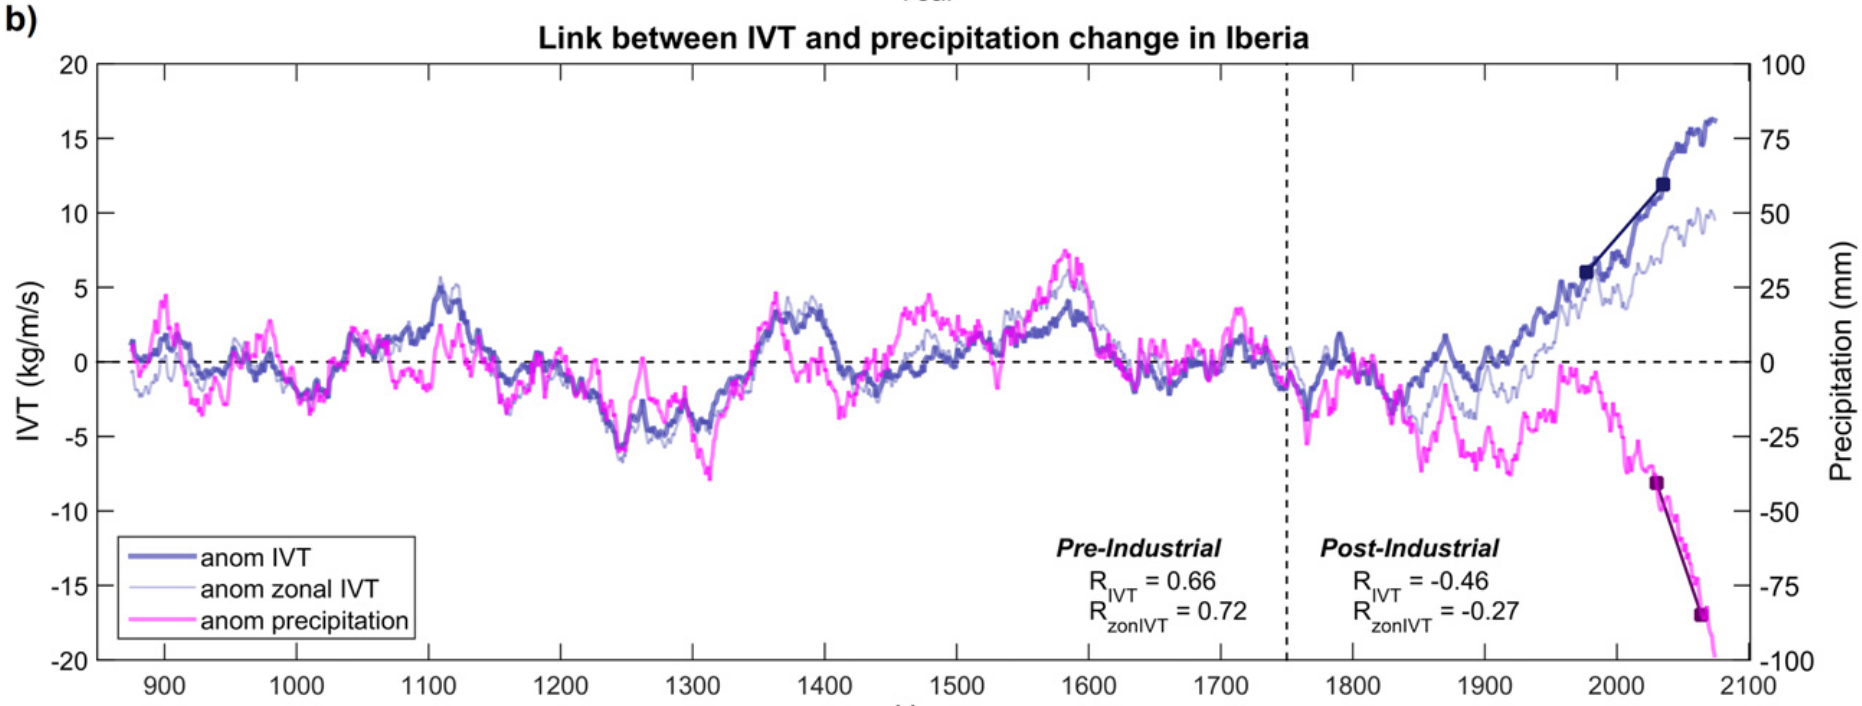
\includegraphics[width=\columnwidth]{imglib/precipitation_iberian_future.png}
    \end{figure}
    
    \begin{figure}[b]
      \centering
      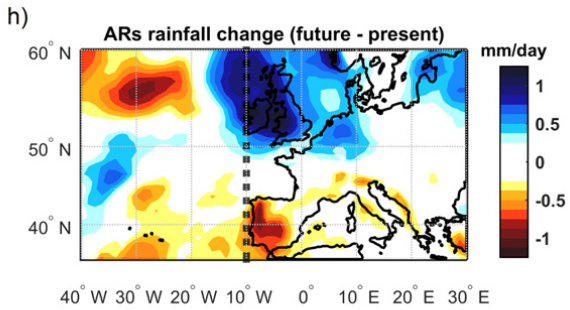
\includegraphics[width=.7\columnwidth]{imglib/ar_rainfall_change.png}
    \end{figure}
   \end{column}
  
 \end{columns} 
\end{frame}
